%!TEX root = presentation.tex
\section{Approche orientée états}

\begin{frame}
	\begin{minipage}{0.5\columnwidth}
		\tableofcontents[
		currentsubsection,
		sectionstyle=show/shaded,
		subsectionstyle=show/show/hide,
		]
	\end{minipage}\hfill
	\begin{minipage}{0.5\columnwidth}
		\inputTikZ{0.7}{img/tikz/approche1.tex}
	\end{minipage}
\end{frame}

\subsection{Architecture hybride orientée états}


\begin{frame}{Quelles sont les architectures possibles dans un EVC ?}
\noindent
		\begin{minipage}{.1\columnwidth}
			\inputTikZ{.7}{img/tikz/legende.tex}
		\end{minipage}
\begin{minipage}{.45\columnwidth}
			\small
			
			\hspace*{1cm}\inputTikZ{0.8}{img/tikz/centralise.tex}
			
			\begin{itemize}
				\item Gestion concurrence/cohérence facilitée
				\item Possible goulot d'étranglement
			\end{itemize}
	\end{minipage}
\begin{minipage}{0.43\columnwidth}
		\only<2>{	\small
			\hspace*{1cm} \inputTikZ{0.8}{img/tikz/decentralise.tex}
			
			\begin{itemize}
				\item Transmission des données directes
				\item Données distribuées
			\end{itemize}}
	\end{minipage}

\only<1>{
	\separatingline{\columnwidth}
\begin{block}{Collaborer plus directement}
	Pourquoi passer par un intermédiaire (serveur) ?
\end{block}
}
\only<2>{
	\separatingline{\columnwidth}
	
\begin{block}{Faciliter la maintenance et le suivi des données}
	Que se passe-t-il s'il n'y a pas de fournisseur de données ?
\end{block}
}
\end{frame}
\begin{frame}{Quelles sont les architectures possibles dans un EVC ?}
\addtocounter{framenumber}{-1}
\begin{minipage}{.5\columnwidth}
	Hybride : Client-serveur + pair-à-pair
	\begin{itemize}
		\item Allègement de la charge du serveur (recherche et récupération)
		\item Répartition des responsabilités (dissémination, stockage)
	\end{itemize}
\end{minipage}\hfill
\begin{minipage}{.5\columnwidth}
		\hspace*{1cm}\inputTikZ{0.8}{img/tikz/semi_centralise.tex}
\end{minipage}

\separatingline{\columnwidth}
	
\begin{block}{Avantages pour la conception 3D sur le web}

	Favoriser les échanges directs 
	
	Augmenter la disponibilité des données
\end{block}
\end{frame}


\begin{frame}{Architecture de communication hybride orientée états 
\cite{Desprat2015a,Desprat2015b}}
\noindent


	\begin{minipage}{.48\columnwidth}
\only<1>{\inputTikZ{1}{img/tikz/archistate.tex}}
\only<2>{\inputTikZ{1}{img/tikz/broadcast.tex}}
	\end{minipage}\hfill
	\begin{minipage}{.48\columnwidth}
	
	Manipule des différentiels d'état ($st_1-st_0$). 
	\begin{itemize}
		\item Client-serveur : Accès \alert{centralisé} aux données pour la 
		persistance 
		long-terme ;
		\item Pair-à-pair : \alert{transmission directe} des données entre les 
		clients pour 
		la 
		collaboration.
	\end{itemize}
	
\end{minipage}
\end{frame}

%\begin{frame}{Modèle de distribution orienté états}
%
%	\begin{minipage}{.4\columnwidth}
%		\begin{figure}
%			\centering
%			\inputTikZ{1}{img/tikz/broadcast.tex}
%			\caption{Emission d'un message par $E$}
%			\label{fig:topo}
%		\end{figure}
%	\end{minipage}\hfill
%	\begin{minipage}{.6\columnwidth}
%		\begin{itemize}
%			\item Typologie de réseau : totalement maillé.
%			\item Message : différentiel entre deux états.
%			\item Cohérence forte : distribution des messages directe aux pairs et au 
%serveur.
%			\item Gestion de la concurrence pessimiste : mécanisme de verrou.
%		\end{itemize}
%	\end{minipage}
%
%\end{frame}


\subsection{3DState}

\begin{frame}{Implémentation de 3DState - Prototype de l'éditeur collaboratif 3D}


	\begin{minipage}{.45\columnwidth}
		Fonctionnalités
		\begin{itemize}
			\item Transformations haut niveau (translation, rotation, homothétie)
			\item Visualisation, navigation
			\item Import de modèles 3D
		\end{itemize}
	
	
	\begin{figure}[h]
		\centering
		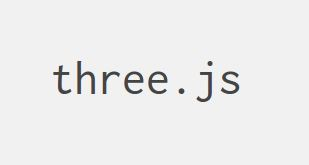
\includegraphics[height=1cm]{img/threejs.jpg}
		
\includegraphics[height=1cm]{img/webgl.png}
		
\includegraphics[height=1cm]{img/js.png}
		\label{fig:client}
	\end{figure}
	\end{minipage}\hfill
	\begin{minipage}{.55\columnwidth}
		\centering
		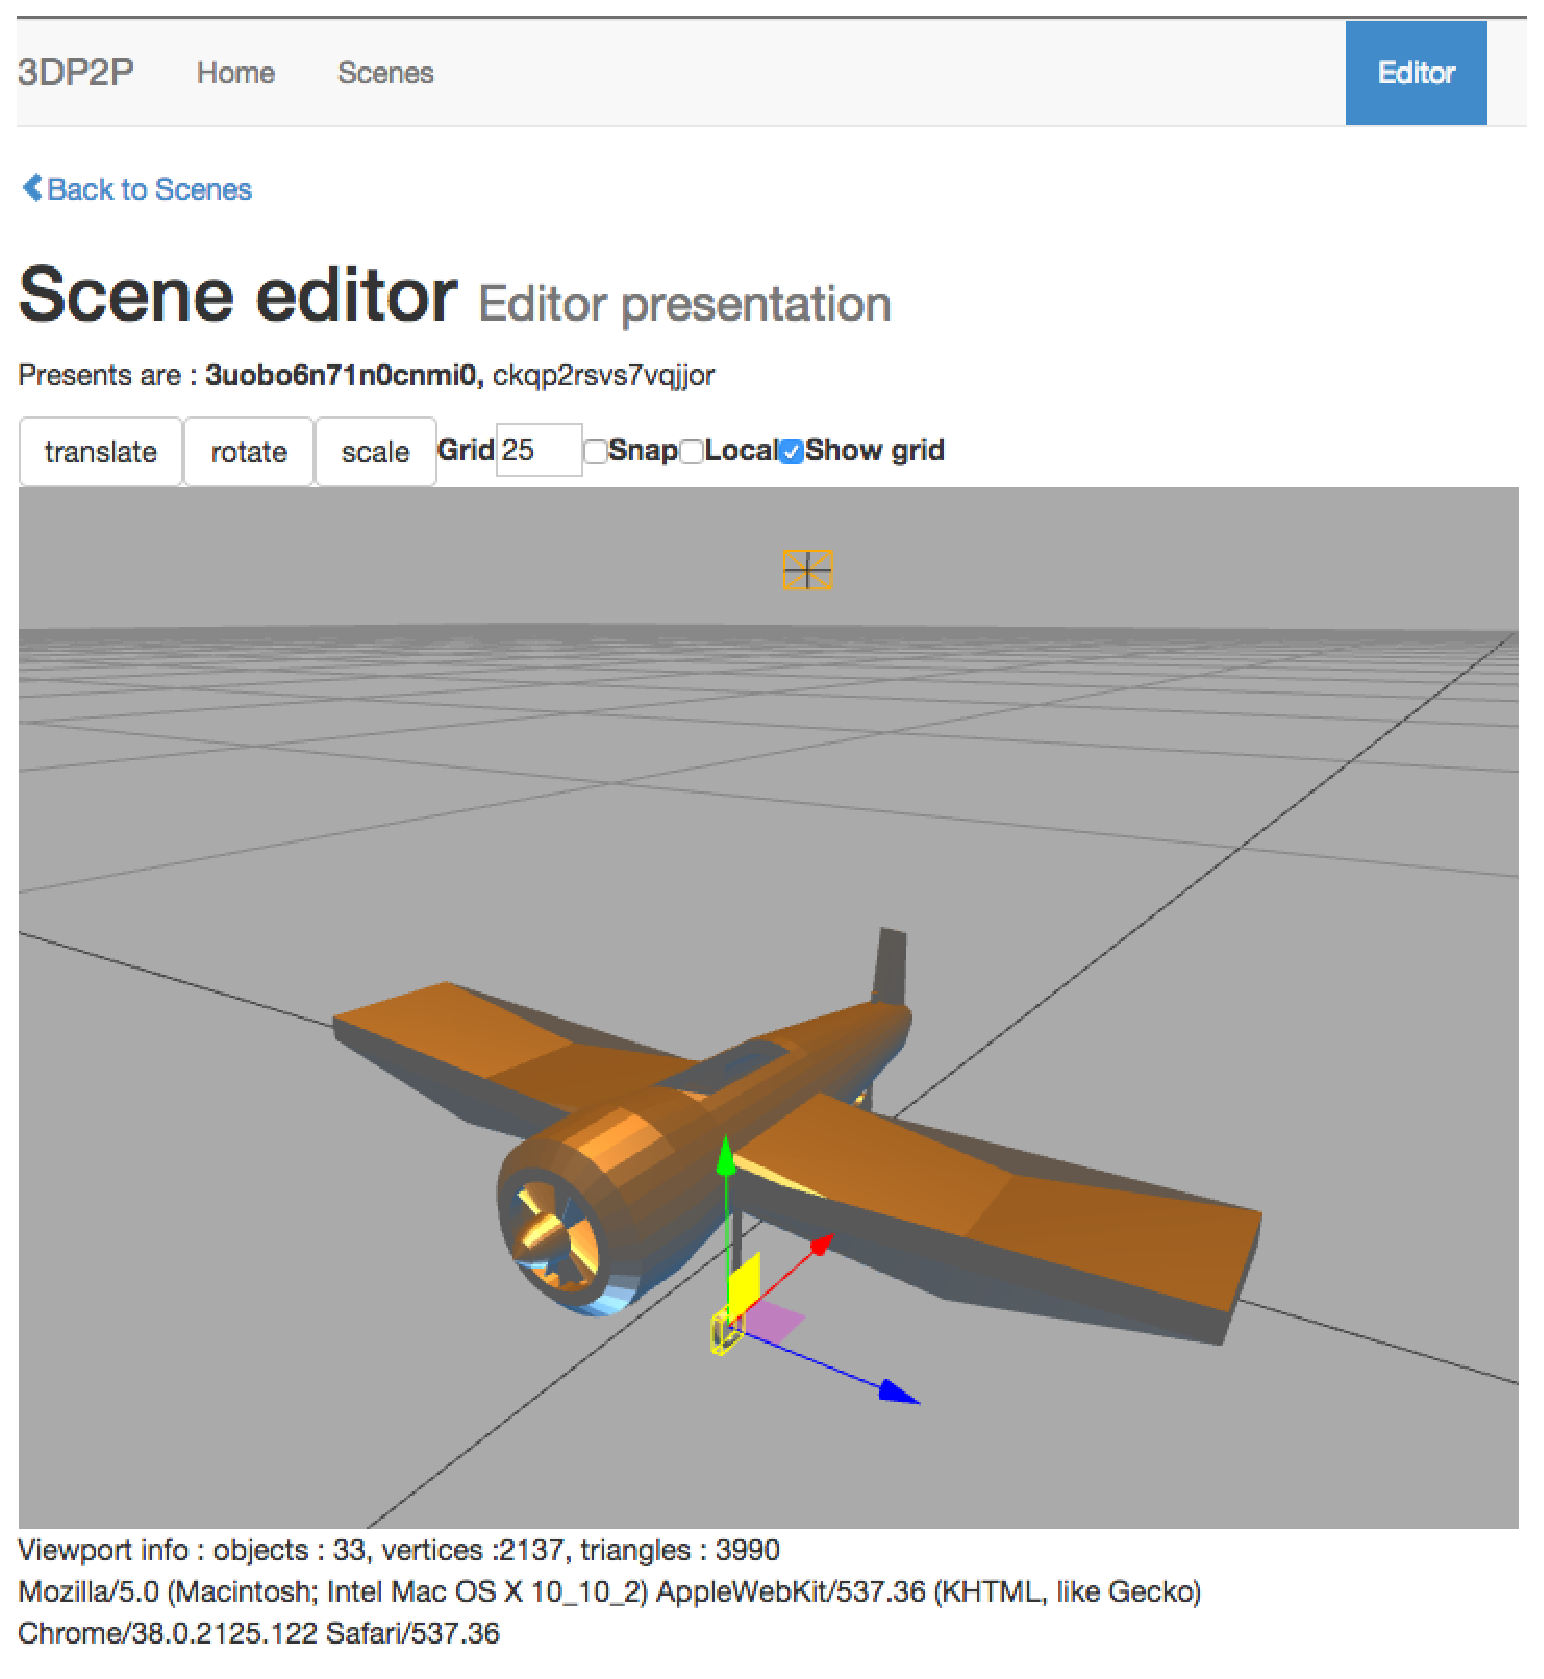
\includegraphics[width=0.8\columnwidth]{eps/editorpresentation.eps}
	\end{minipage}

\end{frame}

\subsection{Expérimentation}

\begin{frame}{Expérimentation approche orientée états}

		\begin{columns}[onlytextwidth]
			\column{0.4\textwidth}
			\begin{alertblock}{Objectif}
				Preuve de faisabilité concernant l'architecture proposée. \\
				Observations des interactions utilisateurs et réseaux\\
				Qualité de la collaboration
			\end{alertblock}
			\column{0.5\textwidth}
			
			\begin{block}{Description}
				Assemblage collaboratif des parties d'un objets.\\
				Type de réseau : réseau local\\
				Prototype : 3DState
			\end{block}
		\end{columns}
		\begin{columns}[onlytextwidth]
			\column{0.4\textwidth}
			\begin{block}{Évaluation}
				Qualité de la collaboration : cohérence, fiabilité, réactivité \\
				Résilience et robustesse du système (situations critiques)
			\end{block}
		
			\column{0.55\textwidth}
			\small
			\begin{table}[!h]
				\caption{Configuration}
				\centering
				\begin{tabular}{lccc}
					\textbf{Essai} & \textbf{Objet} & \textbf{Taille}	& 
					\textbf{NbCollab.}\\ \hline
					Wind turbine			& 6					& 1.0 MB        	& 2 \\ 
					Pick up					& 8					& 1.3 MB         	& 4	\\
					Castle from \textit{server}	& 35				& 1.3 MB        	& 4	\\
					Castle from \textit{peer}& 35 & 1.3 MB & 4 \\ \hline
				\end{tabular}
			\end{table}
		\end{columns}
\end{frame}

\begin{frame}{Résultats}
A partir des données des questionnaires et des observations:
\begin{description}
	\item[Interface utilisateur] minimale, manque de retours visuels.
	\item[Manipulation des objets] bonne évaluation sauf lors d'import de fichiers 3D 
	lourds.
	\item[Attrition] n'altère pas la qualité de la collaboration.
	\item[Globalement] Utilisateurs satisfaits (collaboration et des résultats visuels)
	\item[Qualité de la collaboration] est considérée comme \alert{temps-réel} plus 
	qu'interactive.
\end{description}

En cas de déconnexion soudaine : le système offre une bonne résilience.


%	\begin{itemize}
%		\item Croissance exponentielle des connexions
%		\item Pas de granularité 
%		\item Mise à jour du rendu à la réception d'un message.
%		\item Différentiel d'état ne permet pas de connaître l'historique des 
%		manipulations (\textit{active record}).
%	\end{itemize}
%\begin{figure}
%	\centering
%	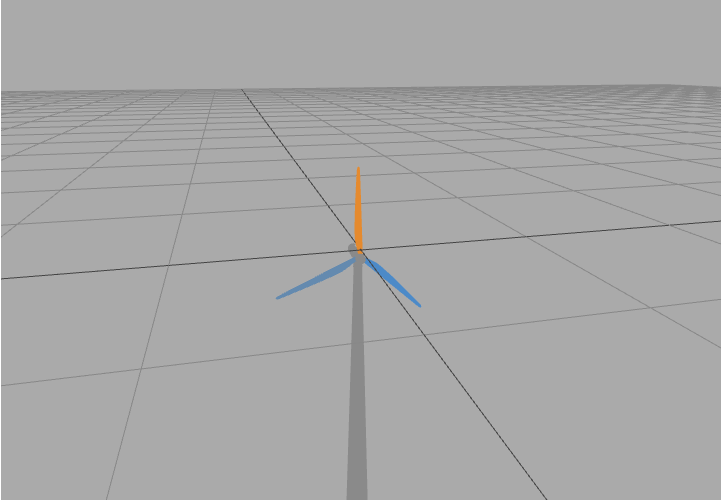
\includegraphics[width=0.3\textwidth]{eps/windturbine.png}
%	\hfill
%	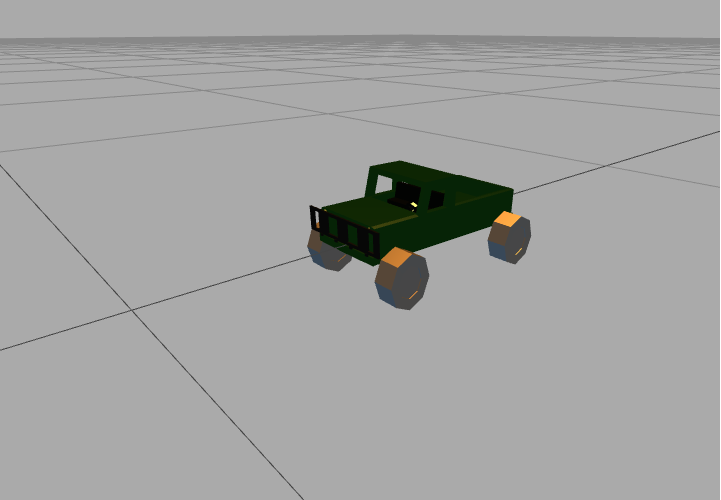
\includegraphics[width=0.3\textwidth]{eps/pickup.png}\hfill
%	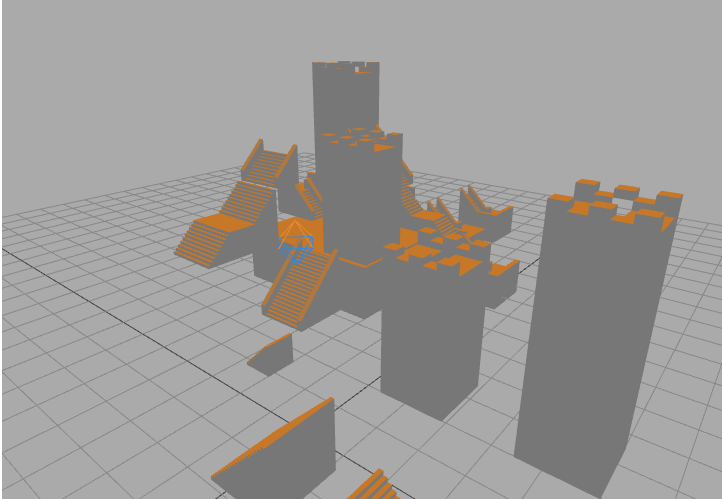
\includegraphics[width=0.3\textwidth]{eps/castle.png}\hfill
%	\caption{\label{screenshots}3D editor's captures during experiments}
%\end{figure}
\end{frame}

\begin{frame}{Bilan de l'approche orientée états}
\begin{table}[]
	\centering
	\begin{tabular}{lcc}
		\hline
		\textbf{QR}              &  \multicolumn{2}{c}{\textbf{Approche orientée états}}  
		\\ \hline
		\textbf{QR1 Réseau}      & \tickpartial   & Topologie complète, 
		diff. état       \\
		\textbf{QR2 Traçabilité} &         \fail                         & 
		Aucune                                    \\
		\textbf{QR3 Autonomie} &  \tickpartial & Stockage local 
		(session)                                 \\
		\textbf{QR4 Validité}    &         \fail                            &  
		Aucune                                     \\
		\textbf{QR5 Métriques}   & \tickpartial (quali.) \fail  (quant.)                         
		&  \multicolumn{1}{c}{\begin{tabular}[c]{@{}c@{}}Cohérence, fiabilité, 
		réactivité.\\ Robutesse et,résilience\end{tabular}}       \\ 
		\hline
	\end{tabular}
\end{table}
	\begin{description}
	\item[QR 1] L'architecture hybride permet d'augmenter la proximité entre les 
	utilisateurs. L'utilisateur est responsable de la transmission des modifications
	
	\item[QR 3] L'utilisateur stocke les informations dont il a besoin sur son client.
	
	\item[QR 5] Architecture faisable. Retours utilisateur positifs même problèmes 
	lors d'imports ou passage à l'échelle
	
	\end{description}
\end{frame}